\cleardoublepage

\chapter{Introduction}
\markboth{Introduction}{Introduction}
%\addcontentsline{toc}{chapter}{Introduction}

\vspace{-1cm}

\section{Motivation}

% Describe preterm birth
Preterm birth  (PTB) --- characterised as birth before 37 full weeks of gestation --- affects an estimated 7\% of births in Switzerland, and 11.1\% of all live births worldwide, which corresponds to nearly 15 million babies per year \citep{Blencowe2013}. 
This comes with a heavy societal burden as it is one of the predominant risk factors behind neurodevelopmental disorders \citep{Pierrat2017,Twilhaar2018}, besides increasing the neonatal and post-discharge costs up to 33 times \citep{Tommiska2003} as compared to term birth. %Economic costs of care in extremely low birth weight infants during the first 2 years of life 
PTB has been associated with a wide range of impairments in cognitive functions spanning attention \citep{Rommel2017}, working memory \citep{Allotey2018}, affective behaviour \citep{Hornman2016}, executive functions \citep{Costa2017, Burnett2018}, among others \citep{Moreira2014, Allotey2018}. 
Often unveiled only when children reach school age, some of these difficulties may persist throughout life \citep{Anderson2014, Kajantie2019}. In Switzerland, while the majority of the patients have positive outcomes, 21\% show some form of cognitive impairment, particularly in short term memory \citep{Pittet-Metrailler2019a}.  Understanding the neurological underpinnings of these difficulties is thus crucial to identify potential interventions and establish critical periods to restore typical development \citep{Wolke2019}.

% Introduce fMRI as an ideal tool to study it
 Functional magnetic resonance imaging (fMRI) is a powerful tool to characterise brain function in a non-invasive fashion and is, therefore, ideal to investigate the neurological basis of clinical outcomes in the young population. Typically relying on the blood oxygenation level dependent signal, it indirectly measures brain activity with exceptional spatial specificity due to its signal reliability, high spatial resolution for a non-invasive method, and reproducibility. Thanks to this technique, it is now known that brain activity intrinsically oscillates in a highly organised way in rest \citep{Damoiseaux2006}, and during performance of tasks \citep{Elliott2019}. This has promoted discoveries linking brain function and the performance of cognitive demanding tasks in several domains of cognitive neuroscience \citep{Raichle2001, Poldrack2012, DEsposito2016}. 
 
FMRI is, in many ways, well-suited to investigate paediatric populations, especially since robust measures of functional activation and connectivity can be obtained from short scanning sessions. It has been successfully employed in studies involving young cohorts tapping into language \citep{Centeno2014, Pigdon2020}, somatomotor \citep{Zwicker2011, Sgandurra2018}, attention \citep{Somandepalli2015, Jiang2019, Harrewijn2020}, memory \citep{Mankinen2015, DeBie2015}, affective processing \citep{Loveland2008, McRae2012}, working memory \citep{Siffredi2017, Yaple2018}, and executive functions \citep{Wang2013, Staphorsius2015}. All of these abilities are more likely to be impaired in preterm- than in term-born individuals, highlighting fMRI's fitness to study this population. Indeed, this technique has uncovered altered brain responses in regions underlying executive functions in preterm-born children in frontal \citep{Reveillon2013,Murner-Lavanchy2014} and temporal areas \citep{Kwon2014a, Wilke2014} which were linked to impaired language performance at age 14\textendash15 \citep{Wilke2014}.
  
Recently, fMRI studies have shown that the brain activity is highly dynamic, fluctuating between large-scale brain states formed by simultaneous activation of different subsets of brain regions during rest \citep{Chang2010, Preti2017, Liu2018} and task performance \citep{Di2015, Cheng2018}. Crucially, features of these moment-to-moment fluctuations of brain configuration have very recently been discovered to be linked to cognitive ability in humans, both during rest \cite{Chen2019} and while performing attentional tasks \cite{Fong2019}. These findings indicate the high potential of brain dynamics as an avenue to further characterise the effects of prematurity in the brain, additionally shedding light on how they relate to cognitive outcomes in those who were born too soon. 
 


\section{Organization and main contributions}

% Summary of all chapters

The goal of this thesis has been to advance the knowledge on the neural effects of preterm birth in the resting state as well as during performance of cognitive tasks. This manuscript is thus organised as a compilation of two published articles and three preprints in preparation for submission. 
Chapter \ref{chapter:ch2} provides an overview of the state of the art in functional MRI analysis and preterm birth research, and serves as a background for the studies presented in subsequent chapters. 
It starts by introducing fMRI as a powerful tool to investigate human brain function, followed by a description of currently available methodologies for human brain mapping using this technique. 
It then characterises the clinical aspects of preterm birth and presents the current knowledge on how its outcomes relate to brain function.
Chapters \ref{chapter:ch3}, \ref{chapter:ch4} and \ref{chapter:ch5}, reproduce published manuscripts and articles in preparation which contribute both through novel research, as well as complementary analyses to existing knowledge.  
Chapter \ref{chapter:ch6} then summarises and integrates the results, and proposes avenues for future research. 

% Disclaimer – use of pronoun "we" intead of "I"
Below, I summarise the main research questions and contributions of each article. 
In all of them I contributed to the planning, performed all data processing and analysis as well as methods development and statistical analysis where applicable, wrote --- or contributed equally to the writing of --- the manuscript and revisions. 
Since all of these studies were achieved thanks to a collaboration involving large groups of people, I will use the personal pronoun "we" from now on when discussing the work done. 



\begin{figure}[h!]
\centering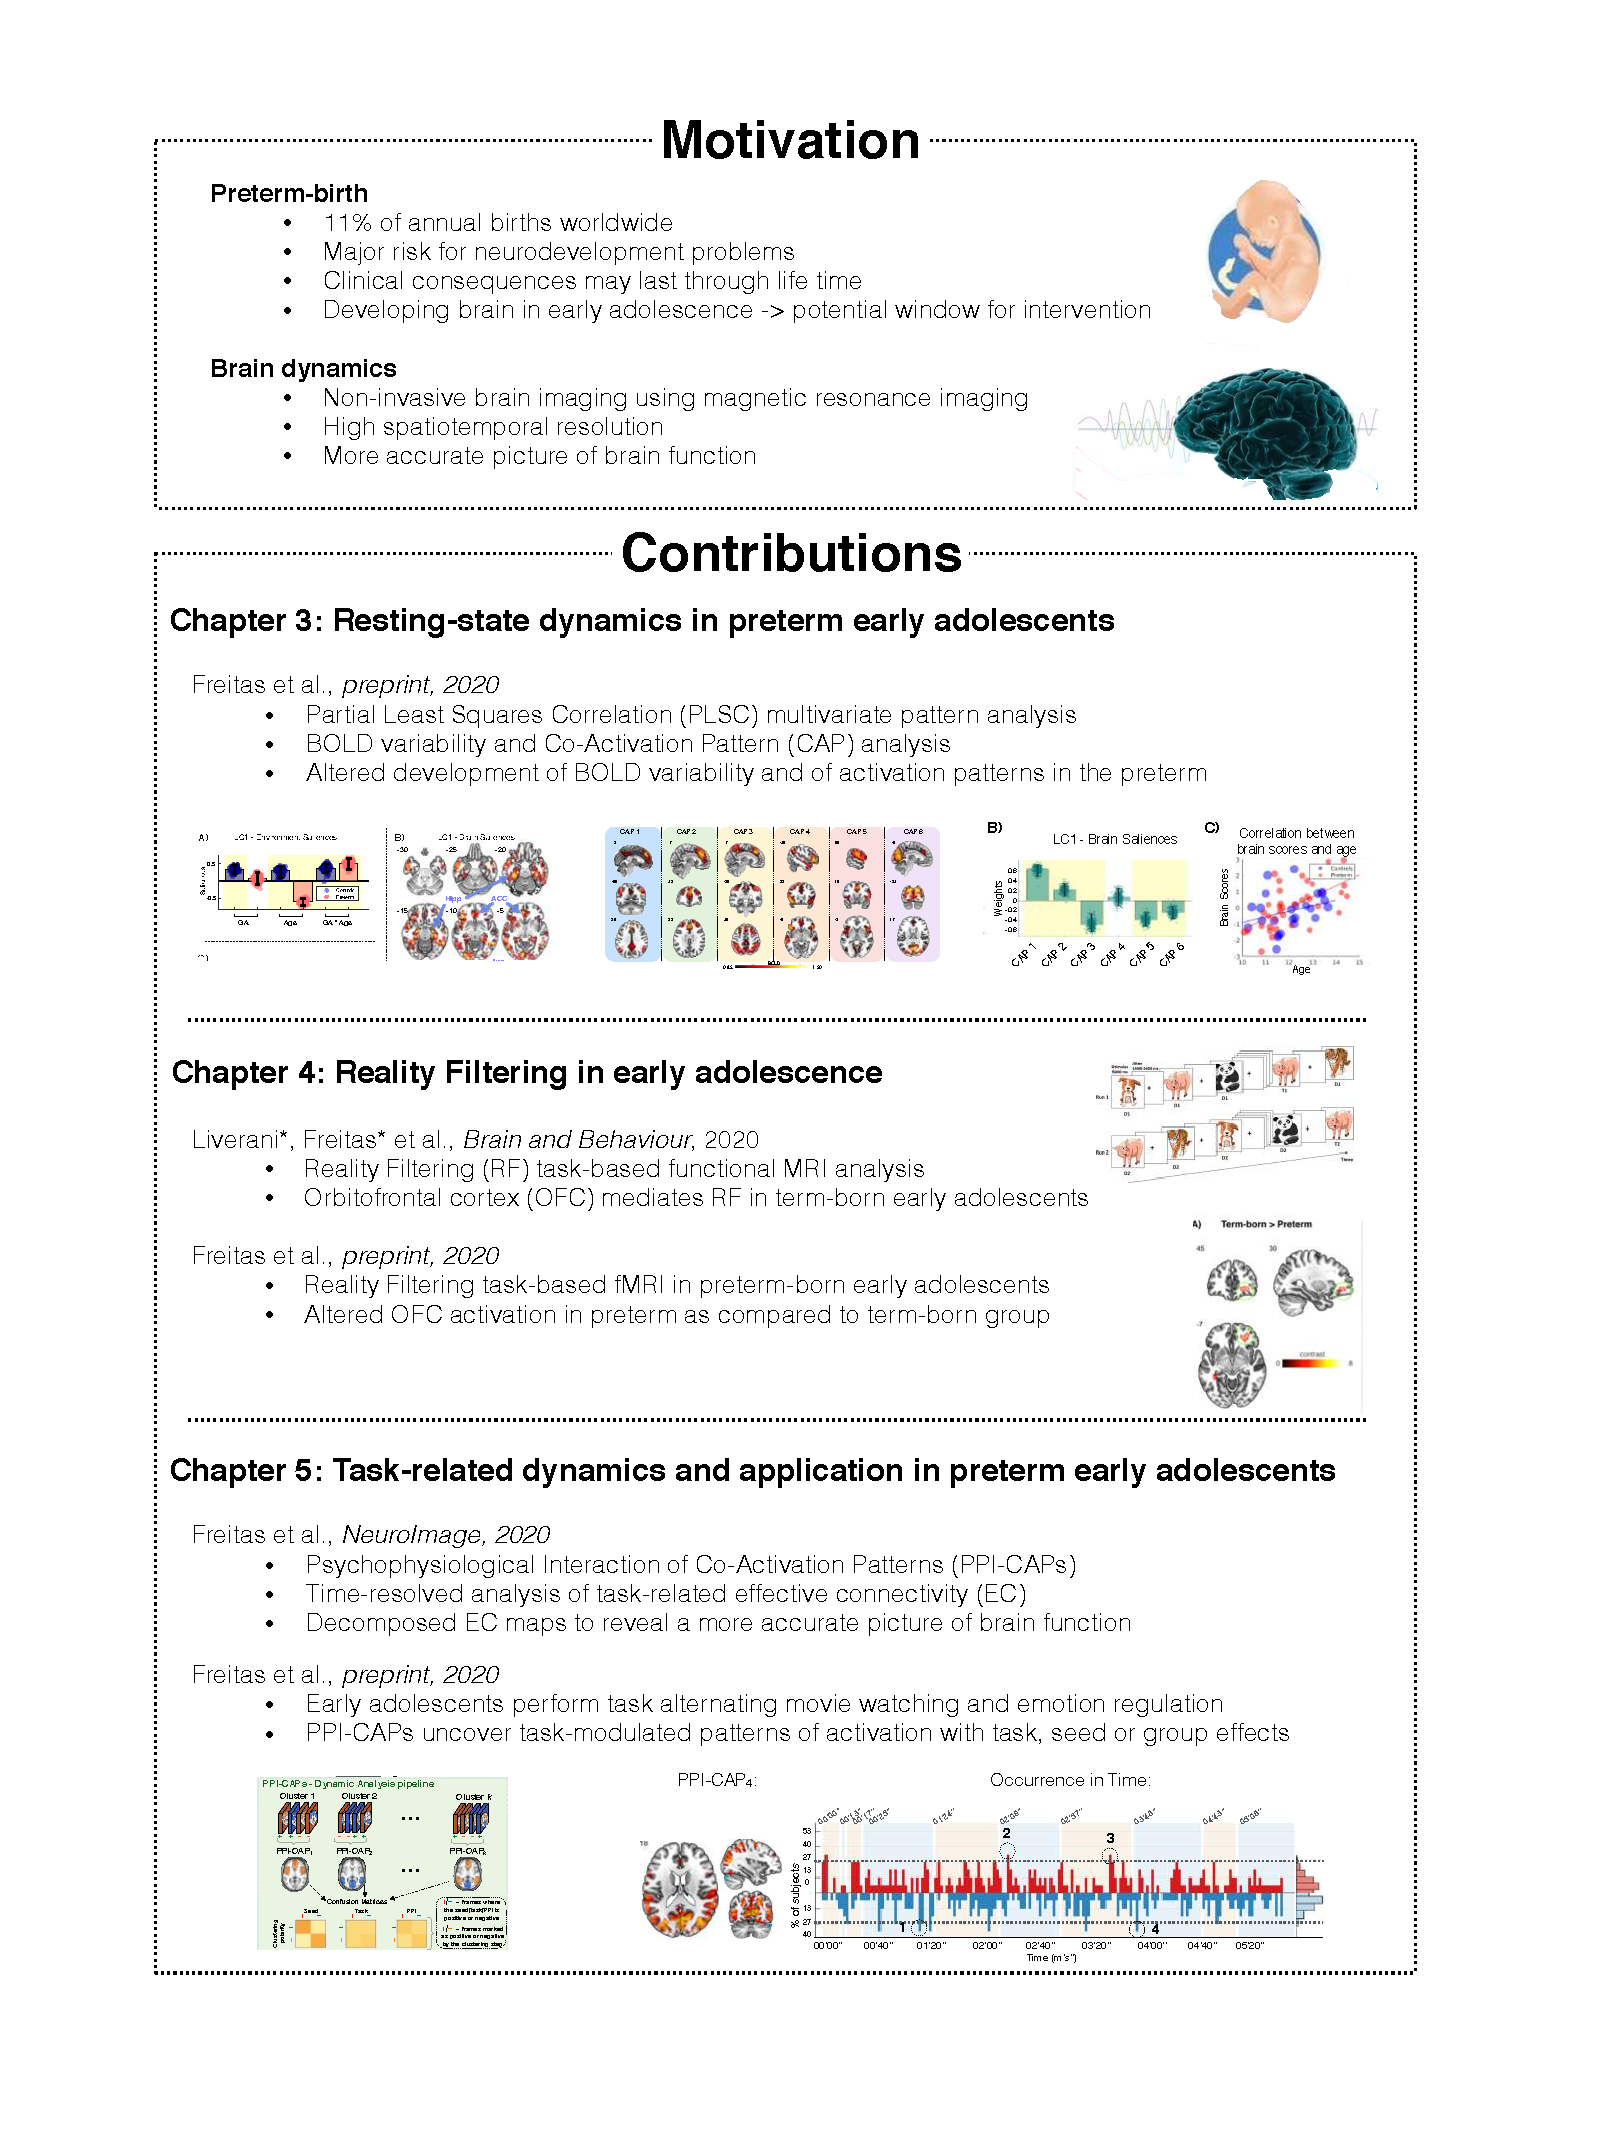
\includegraphics[width=0.95\linewidth]{images/Ch1/Overview.pdf}
\caption{\textbf{Thesis overview.} Main contributions on brain dynamics in preterm-birth. } \label{fig:overview}
\end{figure}


\subsection*{Chapter \ref{chapter:ch3}: BOLD signal variability and dynamic spontaneous brain function in the preterm-born}
Although brain analysis methods often rely on measuring and comparing the average activity in certain areas of interest, blood oxygenation level dependent (BOLD) signal variability has been shown to yield additional information on brain function that is linked to cognitive abilities.
To the best of my knowledge, no one has investigated BOLD signal variability in preterm-born populations. In this chapter, I look into functional brain dynamics in two ways: first, in terms of voxelwise BOLD signal variability and its relationship with gestational age and age at assessment. Secondly, I perform a seed-based co-activation pattern analysis focusing on the dorsal anterior cingulate cortex, an area previously described to be affected by preterm-birth \citep{White2014,Daamen2015,Lordier2019} that was also highlighted in the analysis of BOLD variability. 

\subsubsection*{Section \ref{section:ch3_BOLDvar_paper}: \textit{(Journal Article)} Altered BOLD variability development and brain dynamics in preterm-born young adolescents}
\textit{Is the development of BOLD signal variability affected by preterm birth?}\\
\textit{Does preterm birth affect finer temporal scale brain dynamics?}

BOLD signal variability, calculated as the standard deviation of BOLD signal time series, is a measure of how dynamic brain activity is throughout the duration of an fMRI experiment. It has been shown to change with age and cognitive ability \citep{Garrett2013} and to be altered in clinical populations \citep{Zoller2017,Nomi2018, Easson2019}. These studies support its role in reflecting the brain's dynamic range and complexity and, when present at the optimal levels, in allowing greater flexibility for brain function \citep{McIntosh2010, Deco2011}. It is thus a promising avenue to investigate brain "dynamism" in preterm populations. 

In this article, I investigate the link between dynamic brain function and gestational age, as well as with age at assessment, using a multivariate partial least squares (PLS) approach in a resting-state fMRI paradigm. I have addressed this in two steps: First, I compare how those relationships evolve during early adolescence in a preterm-born and a fullterm control group of children. Then, because BOLD variability is closely linked to functional connectivity, I delve deeper into how the relationship between a region of interest identified in this analysis --- namely, the anterior cingulate cortex --- and other parts of the brain evolve over time in these two groups by using co-activation patterns as brain measures for the PLS. We identify interesting interactions between age at assessment and gestational age in both analyses, suggesting that preterm birth alters the development of dynamism in the brain at later stages in life. 


% Description of Chapter 4 - ORFi?
\subsection*{Chapter \ref{chapter:ch4}: Studying cognition with task-based fMRI: Reality Filtering in young populations}

While resting-state analyses provide profound insight into brain function, task-based fMRI paradigms are crucial to understand how the brain works under specific cognitive demands. In the case of preterm populations, there is especial interest in cognitive functions involving frontal brain areas, as neuroimaging studies have highlighted widespread alterations in prefrontal cortex's structure and function in preterm individuals across lifetime. In this chapter, we thus employ a Reality Filtering (RF) task, known to recruit the orbitofrontal cortex (OFC) in adults, to study brain function in this area in young adolescents. To the best of our knowledge, no one has looked into brain function related to RF in children so far. Therefore, this chapter is divided in two steps: First, we confirm the OFC's involvement in RF in typically developing, fullterm-born children. Then, we look into whole-brain, as well as OFC-seed differences, between a preterm-born and a control group while performing an RF task.

\subsection*{Section \ref{section:ch4_orfi_ctrl}: \textit{(Journal Article)} "Get real: orbitofrontal cortex mediates the ability to sense reality in early adolescents"}
\textit{What are the neural processes underlying reality filtering in early adolescents?}

The typical approach to understand the neural underpinnings of cognition is to investigate how brain function changes as a direct effect from task performance. Here, we focus our study on the orbitofrontal cortex (OFC), known to be crucial for the ability to sense reality in adults but to be still under development in young adolescents, to understand how activation in this area changes in the latter population depending on stimuli presentation. Using a previously validated task paradigm adapted to children we confirmed, for the first time using fMRI and in young adolescents, that the OFC mediates reality filtering already at this age.

\subsection*{Section \ref{section:ch4_orfi_groups}: \textit{(Journal Article)} Altered orbitofrontal activation in preterm-born young adolescents during performance of a reality filtering task}
\textit{Are preterm-born young adolescents able to perform a reality filtering task?}\\
\textit{What are the neural processes underlying reality filtering in preterm-born young adolescents?}

Because the prefrontal cortex ––– of which the OFC is a constituting part ---  is known to be affected by preterm birth in several ways, we wanted to investigate both whether preterm-born young adolescents are capable of reality filtering and, if this is the case, whether the OFC is involved. Using the same task as in the previous section, we found that although children in the preterm group were able to perform the task with comparable accuracy to the fullterm group, the levels of OFC activation in the former group are lower and no other regions were more activated than in controls. This suggests that preterm-born individuals may have developed mechanisms to optimise OFC activity such that they are still able to perform the task without depending on the same level of activation as the control group.


% Description of Chapter 5 - PPI-CAPs paper?
\subsection*{Chapter \ref{chapter:ch5}: Time-resolved brain dynamics during task performance}

While typical task-based studies compare and contrast how brain activity changes between different task contexts, they still mostly assume stationary within task blocks. This provides a limited, incomplete snapshot of how the brain works under these circumstances. Resting-state fMRI has benefited from methods that uncover dynamic features of large-scale neuronal function for over a decade \citep{Chang2010}, but task-based paradigms have only recently started to explore this important avenue \citep{Gonzalez-Castillo2018}.

\subsection*{Section \ref{section:ppicaps_method}: \textit{(Journal Article)} "Time-Resolved Effective Connectivity in Task fMRI: Psychophysiological Interactions of Co-Activation Patterns"}
\textit{Can we capture relevant task-related functional dynamics in a frame-wise way?}

% Useful for defense: https://lib.ugent.be/fulltxt/RUG01/002/508/649/RUG01-002508649_2018_0001_AC.pdf

Previous studies have shown that relevant information on brain function is condensed in specific moments of high amplitude peaks in the BOLD signal \citep{Tagliazucchi2011a}, meaning that large parts of the fMRI time series contain information that does not necessarily add information for certain analyses. This means the fMRI data can reduce to a point-process \citep{Tagliazucchi2012} characterised by a sequence of time points when a seed signal traverses a given threshold. If these points are then averaged, one obtains patterns of co-activation with a seed that are recurring throughout the experiment, at a single-frame resolution \citep{Liu2013}.

In this article I develop a seed-based method called Psychophysiological Interactions of Co-Activation Patterns (PPI-CAPs) to investigate such dynamic modulations of functional brain connectivity in a task-based context. In a naturalistic setting where participants watched a TV program, several patterns of co-activation were yielded using a posterior cingulate cortex seed --- chosen due to its well documented connectivity arrangements \citep{Liu2013a, Karahanoglu2015a,Lin2017} and description as a hub region \citep{Andrews-hanna2010} ---, whose occurrence rates and polarity varied depending on the context; on the seed activity; or on an interaction between the two. Moreover, this method exposed the consistency in effective connectivity patterns across subjects and time, allowing us to uncover links between PPI-CAPs and specific stimuli contained in the video. The main contribution of this study was revealing that explicitly tracking connectivity pattern transients is paramount to advance our understanding of how different brain areas dynamically communicate when presented with a set of cues. Given its ability to concentrate the analysis on very limited amounts of data, this represents a promising avenue for further study of dynamic features of task-modulated brain function in clinical or young populations, such as the preterm-born young adolescents most of this thesis concentrates on. 


\subsection*{Section \ref{section:ppicaps_preterm}: \textit{(Journal Article)} "Tracking moment-to-moment functional connectivity in preterm-born young adolescents during movie watching and emotion regulation"}
\textit{Do preterm-born young adolescents present altered configurations of task-related functional dynamics as compared to fullterm-born controls?}

Having shown that PPI-CAPs is a compelling avenue for the study of dynamic features of context-driven brain function in clinical populations \citep{Freitas2020} in Section \ref{section:ppicaps_method}, I then proceed to employ this approach to study dynamic connectivity in preterm-born young adolescents as compared to age-matched controls. To this end, our participants undergo a block-type task which alternates between moments of movie watching --- where the films have an emotional valence (\textit{i.e.}, amusing or repulsive) to them ---  followed by moments of emotion regulation and concentration on their own breathing. We recover six robust and reoccurring patterns of co-activation with a dorsal anterior cingulate cortex seed. Moreover, we show that several of the data-driven patterns have a seed, task, or group main effects, as well as interactions between those. This study further highlights the importance of investigating task-driven brain dynamics in the context of clinical populations to obtain a more accurate picture of healthy and altered brain function.